\documentclass[border=10pt]{standalone}
\usepackage{amsmath}
\usepackage{amssymb}
\usepackage{tikz}
\usetikzlibrary{positioning, arrows.meta, shapes, calc}

\definecolor{neuralblue}{RGB}{70, 130, 180}
\definecolor{sigmoidgreen}{RGB}{60, 179, 113}
\definecolor{softmaxpurple}{RGB}{147, 112, 219}
\definecolor{outputorange}{RGB}{255, 140, 0}

\begin{document}

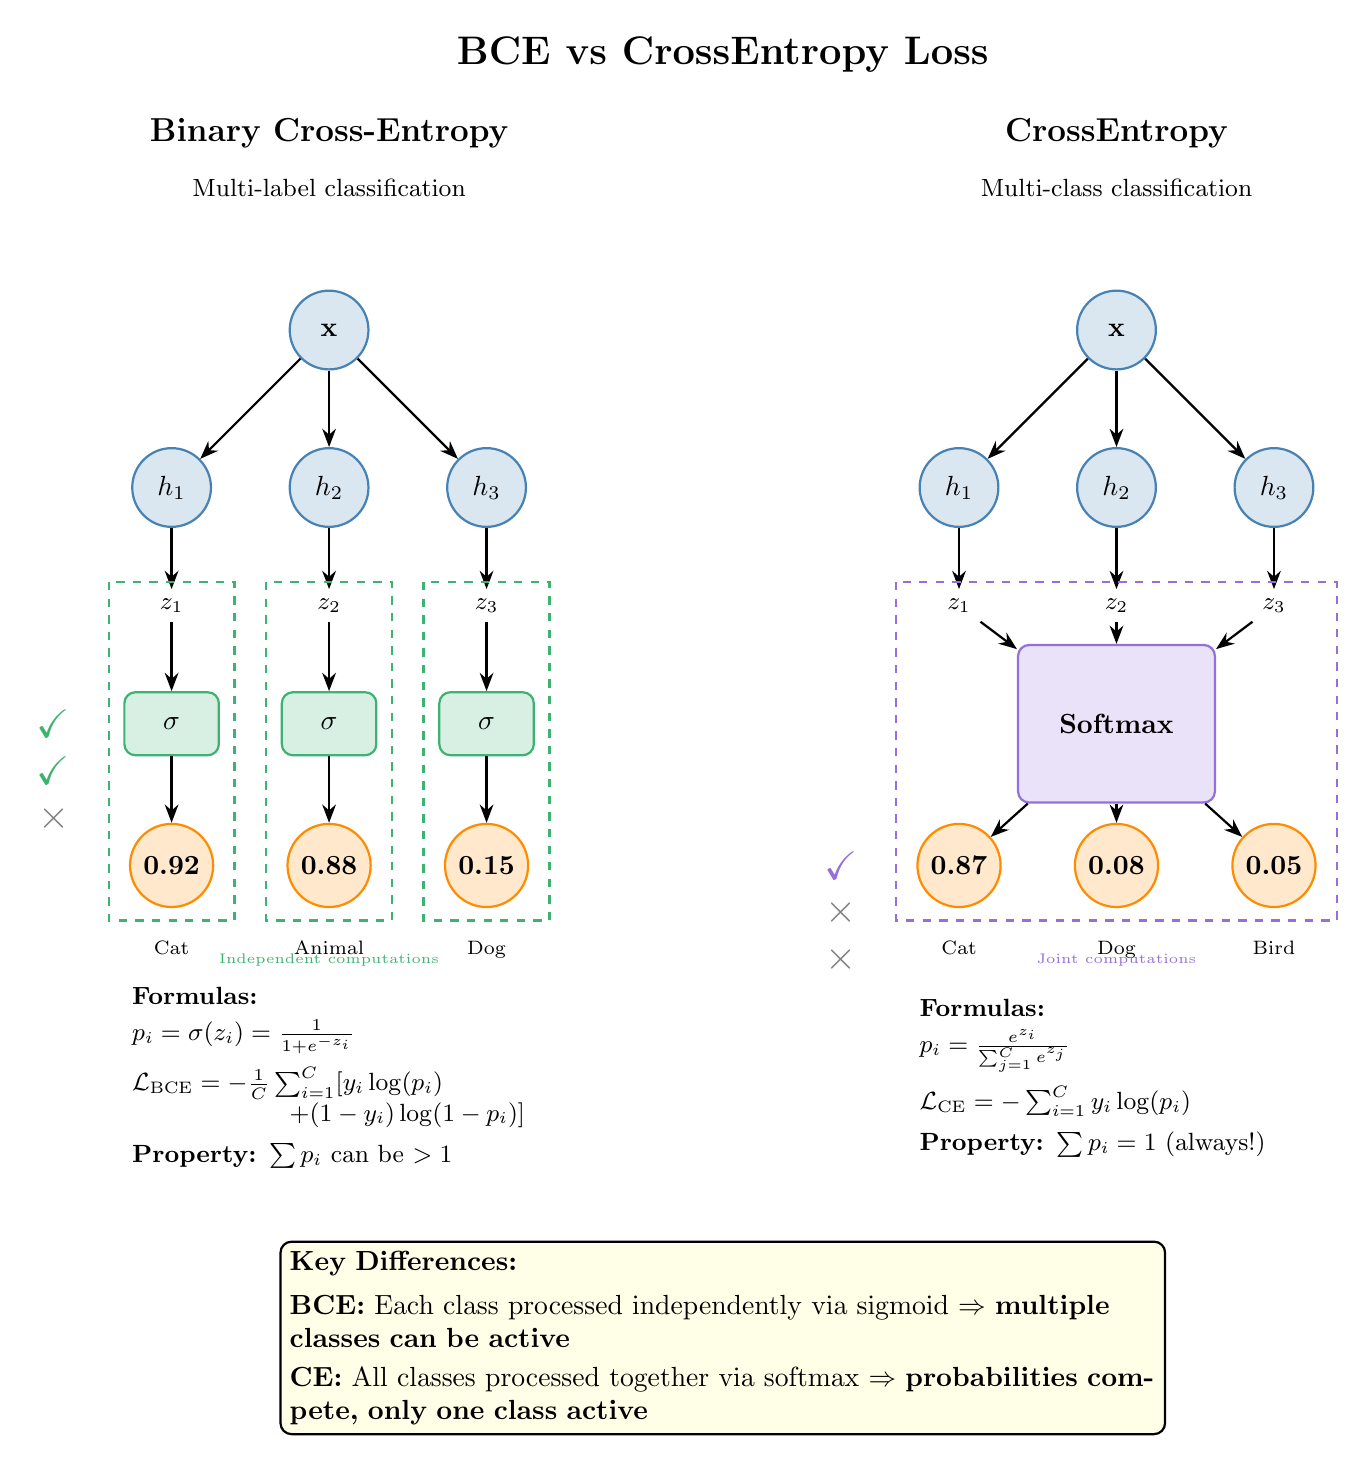
\begin{tikzpicture}[
    node distance=1.5cm,
    neuron/.style={circle, draw=neuralblue, thick, fill=neuralblue!20, minimum size=1cm},
    sigmoid/.style={rectangle, draw=sigmoidgreen, thick, fill=sigmoidgreen!20, minimum width=1.2cm, minimum height=0.8cm, rounded corners},
    softmax/.style={rectangle, draw=softmaxpurple, thick, fill=softmaxpurple!20, minimum width=2.5cm, minimum height=2cm, rounded corners},
    output/.style={circle, draw=outputorange, thick, fill=outputorange!20, minimum size=1cm},
    arrow/.style={-Stealth, thick},
    label/.style={font=\small}
]

% Title
\node[font=\Large\bfseries] at (0, 8.5) {BCE vs CrossEntropy Loss};

% ============ LEFT SIDE: BCE ============
\node[font=\large\bfseries] at (-5, 7.5) {Binary Cross-Entropy};
\node[font=\small, text width=5cm, align=center] at (-5, 6.8) {Multi-label classification};

% Input layer
\node[neuron] (bce-input) at (-5, 5) {$\mathbf{x}$};

% Hidden representation
\node[neuron] (bce-hidden1) at (-7, 3) {$h_1$};
\node[neuron] (bce-hidden2) at (-5, 3) {$h_2$};
\node[neuron] (bce-hidden3) at (-3, 3) {$h_3$};

% Logits
\node[label] (bce-logit1) at (-7, 1.5) {$z_1$};
\node[label] (bce-logit2) at (-5, 1.5) {$z_2$};
\node[label] (bce-logit3) at (-3, 1.5) {$z_3$};

% Sigmoid nodes
\node[sigmoid] (bce-sig1) at (-7, 0) {$\sigma$};
\node[sigmoid] (bce-sig2) at (-5, 0) {$\sigma$};
\node[sigmoid] (bce-sig3) at (-3, 0) {$\sigma$};

% Outputs
\node[output] (bce-out1) at (-7, -1.8) {\textbf{0.92}};
\node[output] (bce-out2) at (-5, -1.8) {\textbf{0.88}};
\node[output] (bce-out3) at (-3, -1.8) {\textbf{0.15}};

% Labels
\node[label, below=0.3cm of bce-out1, font=\scriptsize] {Cat};
\node[label, below=0.3cm of bce-out2, font=\scriptsize] {Animal};
\node[label, below=0.3cm of bce-out3, font=\scriptsize] {Dog};

% Arrows
\draw[arrow] (bce-input) -- (bce-hidden1);
\draw[arrow] (bce-input) -- (bce-hidden2);
\draw[arrow] (bce-input) -- (bce-hidden3);

\draw[arrow] (bce-hidden1) -- (bce-logit1);
\draw[arrow] (bce-hidden2) -- (bce-logit2);
\draw[arrow] (bce-hidden3) -- (bce-logit3);

\draw[arrow] (bce-logit1) -- (bce-sig1);
\draw[arrow] (bce-logit2) -- (bce-sig2);
\draw[arrow] (bce-logit3) -- (bce-sig3);

\draw[arrow] (bce-sig1) -- (bce-out1);
\draw[arrow] (bce-sig2) -- (bce-out2);
\draw[arrow] (bce-sig3) -- (bce-out3);

% Independent processing boxes
\draw[dashed, sigmoidgreen, thick] (-7.8, 1.8) rectangle (-6.2, -2.5);
\draw[dashed, sigmoidgreen, thick] (-5.8, 1.8) rectangle (-4.2, -2.5);
\draw[dashed, sigmoidgreen, thick] (-3.8, 1.8) rectangle (-2.2, -2.5);

\node[font=\tiny, sigmoidgreen] at (-5, -3) {Independent computations};

% Formulas for BCE
\node[font=\small, text width=5cm, align=left] at (-5, -4.5) {
    \textbf{Formulas:} \\[2pt]
    $p_i = \sigma(z_i) = \frac{1}{1 + e^{-z_i}}$ \\[4pt]
    $\mathcal{L}_{\text{BCE}} = -\frac{1}{C}\sum_{i=1}^{C} [y_i \log(p_i)$\\ \hspace{2cm}$+ (1-y_i)\log(1-p_i)]$ \\[4pt]
    \textbf{Property:} $\sum p_i$ can be $> 1$
};

% ============ RIGHT SIDE: CrossEntropy ============
\node[font=\large\bfseries] at (5, 7.5) {CrossEntropy};
\node[font=\small, text width=5cm, align=center] at (5, 6.8) {Multi-class classification};

% Input layer
\node[neuron] (ce-input) at (5, 5) {$\mathbf{x}$};

% Hidden representation
\node[neuron] (ce-hidden1) at (3, 3) {$h_1$};
\node[neuron] (ce-hidden2) at (5, 3) {$h_2$};
\node[neuron] (ce-hidden3) at (7, 3) {$h_3$};

% Logits
\node[label] (ce-logit1) at (3, 1.5) {$z_1$};
\node[label] (ce-logit2) at (5, 1.5) {$z_2$};
\node[label] (ce-logit3) at (7, 1.5) {$z_3$};

% Softmax node (combined)
\node[softmax] (ce-softmax) at (5, 0) {\textbf{Softmax}};

% Outputs
\node[output] (ce-out1) at (3, -1.8) {\textbf{0.87}};
\node[output] (ce-out2) at (5, -1.8) {\textbf{0.08}};
\node[output] (ce-out3) at (7, -1.8) {\textbf{0.05}};

% Labels
\node[label, below=0.3cm of ce-out1, font=\scriptsize] {Cat};
\node[label, below=0.3cm of ce-out2, font=\scriptsize] {Dog};
\node[label, below=0.3cm of ce-out3, font=\scriptsize] {Bird};

% Arrows
\draw[arrow] (ce-input) -- (ce-hidden1);
\draw[arrow] (ce-input) -- (ce-hidden2);
\draw[arrow] (ce-input) -- (ce-hidden3);

\draw[arrow] (ce-hidden1) -- (ce-logit1);
\draw[arrow] (ce-hidden2) -- (ce-logit2);
\draw[arrow] (ce-hidden3) -- (ce-logit3);

\draw[arrow] (ce-logit1) -- (ce-softmax);
\draw[arrow] (ce-logit2) -- (ce-softmax);
\draw[arrow] (ce-logit3) -- (ce-softmax);

\draw[arrow] (ce-softmax) -- (ce-out1);
\draw[arrow] (ce-softmax) -- (ce-out2);
\draw[arrow] (ce-softmax) -- (ce-out3);

% Joint processing box
\draw[dashed, softmaxpurple, thick] (2.2, 1.8) rectangle (7.8, -2.5);
\node[font=\tiny, softmaxpurple] at (5, -3) {Joint computations};

% Formulas for CE
\node[font=\small, text width=5cm, align=left] at (5, -4.5) {
    \textbf{Formulas:} \\[2pt]
    $p_i = \frac{e^{z_i}}{\sum_{j=1}^{C} e^{z_j}}$ \\[4pt]
    $\mathcal{L}_{\text{CE}} = -\sum_{i=1}^{C} y_i \log(p_i)$ \\[4pt]
    \textbf{Property:} $\sum p_i = 1$ (always!)
};

% ============ KEY DIFFERENCES BOX ============
\node[draw, thick, fill=yellow!10, text width=11cm, align=left, rounded corners] at (0, -7.8) {
    \textbf{Key Differences:} \\[4pt]
    \textbf{BCE:} Each class processed independently via sigmoid $\Rightarrow$ \textbf{multiple classes can be active} \\[2pt]
    \textbf{CE:} All classes processed together via softmax $\Rightarrow$ \textbf{probabilities compete, only one class active}
};

% Visual indicators for multiple active classes (BCE)
\node[font=\Large, sigmoidgreen] at (-8.5, 0) {$\checkmark$};
\node[font=\Large, sigmoidgreen] at (-8.5, -0.6) {$\checkmark$};
\node[font=\Large, gray] at (-8.5, -1.2) {$\times$};

% Visual indicators for single active class (CE)
\node[font=\Large, softmaxpurple] at (1.5, -1.8) {$\checkmark$};
\node[font=\Large, gray] at (1.5, -2.4) {$\times$};
\node[font=\Large, gray] at (1.5, -3.0) {$\times$};

\end{tikzpicture}

\end{document}
